% Format teze zasnovan je na paketu memoir
% http://tug.ctan.org/macros/latex/contrib/memoir/memman.pdf ili
% http://texdoc.net/texmf-dist/doc/latex/memoir/memman.pdf
% 
% Prilikom zadavanja klase memoir, navedenim opcijama se podešava 
% veličina slova (12pt) i jednostrano štampanje (oneside).
% Ove parametre možete menjati samo ako pravite nezvanične verzije
% mastera za privatnu upotrebu (na primer, u b5 varijanti ima smisla 
% smanjiti 
\documentclass[12pt,oneside]{memoir} 

% Paket koji definiše sve specifičnosti master rada Matematičkog fakulteta
\usepackage[latinica]{matfmaster} 
\usepackage{elm-highlighting}
\usepackage{lmodern}
\usepackage{listings,xcolor}

\usepackage[T1]{fontenc}
\usepackage{xcolor}
\usepackage[scaled=0.9]{DejaVuSansMono}

\lstdefinestyle{DOS}
{
    backgroundcolor=\color{black},
    basicstyle=\scriptsize\color{white}\ttfamily
}
\definecolor{commentgreen}{RGB}{2,112,10}
\definecolor{eminence}{RGB}{108,48,130}
\definecolor{weborange}{RGB}{255,165,0}
\definecolor{frenchplum}{RGB}{129,20,83}

\lstdefinelanguage{elixir}{
    morekeywords={case,catch,def,do,else,false,%
        use,alias,receive,timeout,defmacro,defp,%
        for,if,import,defmodule,defprotocol,%
        nil,defmacrop,defoverridable,defimpl,%
        super,fn,raise,true,try,end,with,field,type%
        unless, |>, <-, \}, \{,},
    otherkeywords={->, \%\{, \, (, )},
    sensitive=true,
    morecomment=[l]{\#},
    morecomment=[n]{/*}{*/},
    morecomment=[s][\color{purple}]{:}{\ },
    morestring=[s][\color{orange}]"",
    commentstyle=\color{commentgreen},
    keywordstyle=\color{eminence},
    stringstyle=\color{red},
	basicstyle=\ttfamily,
	breaklines,
	showstringspaces=false,
	frame=tb
}


%

%

%
% Opcija [biblatex]:
%   ako želite da koristite reference na više jezika i umesto paketa
%   bibtex da koristite BibLaTeX/Biber, dodajte opciju "biblatex" tj.
%   prethodni paket uključite pomoću: \usepackage[biblatex]{matfmaster}
%
% Opcija [b5paper]:
%   ako želite da napravite verziju teze u manjem (b5) formatu, navedite
%   opciju "b5paper", tj. prethodni paket uključite pomoću: 
%   \usepackage[b5paper]{matfmaster}. Tada ima smisla razmisliti o promeni
%   veličine slova (izmenom opcije 12pt na 11pt u \documentclass{memoir}).
%
% Naravno, opcije je moguće kombinovati.
% Npr. \usepackage[b5paper,biblatex]{matfmaster}


% Datoteka sa literaturom u BibTex tj. BibLaTeX/Biber formatu
\bib{matfmaster-primer}

% Ime kandidata na srpskom jeziku (u odabranom pismu)
\autor{Ana Petrović}
% Naslov teze na srpskom jeziku (u odabranom pismu)
\naslov{Testiranje funkcionalnog koda}
% Godina u kojoj je teza predana komisiji
\godina{2023}
% Ime i afilijacija mentora (u odabranom pismu)
\mentor{dr Ime\textsc{Prezime}, redovan profesor\\ Univerzitet u Beogradu, Matematički fakultet}
% Ime i afilijacija prvog člana komisije (u odabranom pismu)
\komisijaA{dr Ime \textsc{Prezime}, vanredni profesor\\ University of Disneyland, Nedođija}
% Ime i afilijacija drugog člana komisije (u odabranom pismu)
\komisijaB{dr Ime \textsc{Prezime}, docent\\ Univerzitet u Beogradu, Matematički fakultet}
% Ime i afilijacija trećeg člana komisije (opciono)
% \komisijaC{}
% Ime i afilijacija četvrtog člana komisije (opciono)
% \komisijaD{}
% Datum odbrane (odkomentarisati narednu liniju i upisati datum odbrane ako je poznat)
% \datumodbrane{}

% Apstrakt na srpskom jeziku (u odabranom pismu)
\apstr{%
Apstrakt
}

% Ključne reči na srpskom jeziku (u odabranom pismu)
\kljucnereci{funkcionalno programiranje, testiranje, verifikacija softvera, programski jezik Elixir, programski jezik Elm}

\begin{document}
% ==============================================================================
% Uvodni deo teze
\frontmatter
% ==============================================================================
% Naslovna strana
\naslovna
% Strana sa podacima o mentoru i članovima komisije
\komisija
% Strana sa posvetom (u odabranom pismu)
%\posveta{Mami, tati i dedi}
% Strana sa podacima o disertaciji na srpskom jeziku
\apstrakt
% Sadržaj teze
\tableofcontents*

% ==============================================================================
% Glavni deo teze
\mainmatter
% ==============================================================================

% ------------------------------------------------------------------------------
\chapter{Uvod}
% ------------------------------------------------------------------------------
\par
Ovde ide uvod .. ... ..... 
\par uvod uvod

\par sta se nalazi u kom poglavlju...


% ------------------------------------------------------------------------------
\chapter{Funkcionalna paradigma}
\label{chp:uvodnideo}

\par Funkcionalno programiranje je specifičan pristup programiranju, tj. programska paradigma, koja se zasniva na pojmu matematičke funkcije. Programi se kreiraju pomoću izraza i funkcija, bez izmena stanja i podataka \cite{func}. Iz tog razloga, jednostavniji su za razumevanje i otporniji na greške u odnosu na imperativne programe. U slučaju funkcionalnih programskih jezika, osnovna apstrakcija je \textit{funkcija}. Programski stil je deklarativnog tipa i umesto naredbi koriste se izrazi, tako da se izvršavanje programa svodi na evaluaciju izraza. Vrednost izraza je nezavisna od konteksta u kojem se izraz nalazi. Osnovna osobina čistih funkcionalnih jezika (eng. \textit{pure functional programming language}) jeste transparentnost referenci, što kao posledicu ima nepostojanje propratnih efekata. Sa druge strane, nečisti funkcionalni jezici (eng. \textit{impure functional programming language}) su manje elegantni jer dozvoljavaju propratne efekte, koji mogu izazvati suptilne greške i biti teži za razumevanje. Međutim, praktičniji su za specifične vrste zadataka, kao što je programiranje korisničkog interfejsa ili rad sa bazom podataka. 
\par Funkcionalni jezici zasnovani su na \textit{lambda računu} (eng. \textit{$\lambda$-calculus}), čija je osnovna svrha da d\a'a  definiciju izračunljivosti. Pored toga što se smatra prvim funkcionalnim jezikom, lambda račun se naziva i najmanjim programskim jezikom na svetu. Sve što se može izračunati lambda računom smatra se izračunljivim. Ekspresivnost funkcionalnih jezika ekvivalentna je ekspresivnosti Tjuringove mašine \cite{turing}. 

\section{Karakteristike funkcionalnih jezika}
U nastavku su objašnjene neke od najvažnijih osobina jezika funkcionalne paradigme. 

\subsection{Odsustvo promenljivih}
Čisti funkcionalni jezici nemaju stanje koje bi se menjalo tokom izvršavanja programa, pa zbog toga ne podržavaju koncept promenljivih. Da bi postigli mutabilnost, koriste koncepte kao što su lambda izrazi ili rekurzija.  Sa druge strane, nečisti funkcionalni jezici podržavaju i karakteristike drugih programskih paradigmi, te je u okviru njih dozvoljena upotreba promenljivih. Iako su fleksibilniji po tom pitanju, nečisti funkcionalni jezici promovišu imutabilnost kao dobru praksu. 

\subsection{Transparentnost referenci}
Koncept transparetnosti referenci se odnosi na to da je vrednost izraza jedinstveno određena. Izraz se može zameniti svojom vrednošću na bilo kom mestu u programu, bez promene u ponašanju programa. Definicija se može proširiti i na funkcije: funkcija poseduje transparentnost referenci ako pri pozivu sa istim vrednostima argumenata uvek proizvodi isti rezultat. Ponašanje takve funkcije je određeno njenim ulaznim vrednostima. Kao posledica, redosled naredbi u funkcionalnim programskim jezicima nije važan.

\subsection{Čista funkcija}
Čista funkcija (eng. \textit{pure function}) ima dve osnovne karakteristike: 
\begin{itemize}
\item Transparentnost referenci 
\item Imutabilnost 
\end{itemize}
\par Imutabilnost podrazumeva odsustvo propratnih efekata, tj. da čista funkcija ne vrši nikakve izmene nad argumentima, kao ni nad promenljivima. Jedini rezultat čiste funkcije jeste vrednost koju ona vrati. Kao posledica ovoga, funkcionalni programi su laki za debagovanje. Čiste funkcije takođe olakšavaju paralelizaciju i konkurentnost aplikacija. Na osnovu ovako napisanih programa, kompilator lako može da paralelizuje naredbe, sačeka da evaluira rezultate kada budu potrebni, i na kraju da zapamti rezultat, s obzirom na to da se on neće promeniti sve dok ulaz ostaje isti. Kod \ref{lst:pure} prikazuje primer jedne čiste funkcije u programskom jeziku Elixir. 

\begin{lstlisting}[language=elixir, caption={Primer čiste funkcije},captionpos=b, label={lst:pure}]
defmodule Math do 
  def fibonacci(0) do 0 end
  def fibonacci(1) do 1 end
  def fibonacci(n) do fibonacci(n-1) + fibonacci(n-2) end
end

IO.puts Math.fibonacci(9)
\end{lstlisting}

\subsection{Rekurzija}
Za razliku od imperativnog programiranja, kod funkcionalno napisanih programa može se primetiti odsustvo petlji. Funkcije se definišu rekurzivno --- pozivaju same sebe i time postižu ponavljanje izvršavanja. U mnogim slučajevima, umesto rekurzije se koriste funkcije višeg reda.

\subsection{Funkcije kao građani prvog reda}
U funkcionalnim programima, funkcije se smatraju građanima prvog reda (eng. \emph{first class citizen}). To znači da u okviru jezika ne postoje restrikcije po pitanju njihovog kreiranja i korišćenja. Građani prvog reda su entiteti u okviru programskog jezika koji mogu biti:
\begin{itemize}
\item deo nekog izraza
\item dodeljeni nekoj promenljivoj
\item prosleđeni kao argument funkcije
\item povratne vrednosti funkcije
\end{itemize}
Mogućnost prosleđivanja funkcija kao argumenata drugih funkcija je ključna za funkcionalnu paradigmu. 

\subsection{Funkcije višeg reda}
Funkcija višeg reda je funkcija koja kao argument uzima jednu ili više funkcija i/ili ima funkciju kao svoju povratnu vrednost. U funkcionalnom programiranju se intenzivno koriste ovakve funkcije, a po svojoj važnosti se posebno izdvajaju \textit{map}, \textit{filter} i \textit{reduce (fold)}.  Funkcija \textit{map} kao argumente prima funkciju i listu, i zatim primeni datu funkciju na svaki element liste i kao povratnu vrednost proizvodi novu listu. Upotrebom funkcije \textit{filter} mogu se eliminisati neželjeni elementi neke liste --- na osnovu prosleđene funkcije predikata i date liste, \textit{filter} vraća listu sa elementima koji ispunjavaju dati kriterijum. \textit{Fold} prihvata tri argumenta: funkciju spajanja, početnu vrednost i listu. Iznova primenjuje funkciju spajanja na početnu vrednost i datu listu, sve dok se rezultat ne redukuje na jednu vrednost. 
\par Prednost korišćenja ovih funkcija je u paralelnom izvršavanju, s obzirom da funkcionalni programi nemaju stanje. Takođe, daju prilično sažet i čist k$\hat{o}$d. Primer koda \ref{lst:high} pokazuje upotrebu funkcija višeg reda u programskom jeziku Elm.

\begin{lstlisting}[language=elm, caption={Funkcije višeg reda},captionpos=b, label={lst:high}]
[1, 2, 3] |> List.map (\number -> number * 2) -- [2, 4, 6]
[1, 2, 3, 4, 5] |> List.filter (\number -> number <= 3) -- [1, 2, 3]
[1, 2, 3, 4, 5] |> List.foldl (\item total -> total + item) 0 -- 15
\end{lstlisting}


\section{Testiranje uopšteno (smisliti naslov)}
\label{sec:piramid}

\par Testiranje koda je jedan od najvažnijih aspekata u procesu razvoja softvera. Cilj testiranja je pronalaženje grešaka, proverom da li su ispunjeni svi funkcionalni i nefunkcionalni zahtevi \cite{test}.  Softver koji ne radi onako kako je predviđeno može dovesti do različitih problema, kao što su gubitak novca i vremena, ili u najgorim slučajevima --- povrede ili smrti. Testiranjem se osigurava kvalitet softvera i smanjuje rizik od neželjenog ponašanja. Glavna uloga testiranja jeste verifikacija softvera --- provera da li sistem zadovoljava specifikaciju, ali uključuje i validaciju --- proveru da li sistem ispunjava sve potrebe korisnika.  
\par Razvoj vođen testovima (eng. \emph{Test-Driven Development , TDD}) je praksa u razvoju softvera koja nalaže da se prvo napišu testovi. Ti testovi na početku ne prolaze, s obzirom na to da k$\hat{o}$d još uvek nije implementiran, a zatim se iznova pokreću tokom pisanja samog koda, sve dok ne prođu. Ova tehnika kontinualnog testiranja tokom razvoja se često preporučuje jer se lako i veoma rano uoče greške i time sprečavaju u kasnijim fazama razvoja. Ipak, u ovom radu neće biti primenjen TDD pristup. Kako je tema testiranje, fokus nije na pisanju koda aplikacije, već testova za već napisan projekat. Aplikacija koja će biti testirana služi samo kao primer na kome će biti prikazani značajni koncepti testiranja funkcionalnih programa. Kratak opis testiranog projekta biće preciznije objašnjen u poglavlju \ref{chp:msnr}. 

\subsection{Organizacija testova}
\par Model piramide testiranja (prikazan na slici \ref{fig:piramida}) je koncept koji pomaže u razmišljanju o tome kako testirati softver \cite{cohn}. Uloga piramide je da vizuelno predstavi logičku organizaciju standarda u testiranju. Sastoji se od tri sloja: bazu piramide predstavljaju jedinični testovi (eng. \emph{unit test}). Njih bi trebalo da bude najviše --- kako su najmanji, samim tim su i najbrži, a izvršavaju se u potpunoj izolaciji. Na sledećem nivou, u sredini piramide, nalaze se integracioni testovi (ili testovi servisa). Integracija podrazumeva način na koji različite komponente sistema rade zajedno. Nisu potrebne interakcije sa korisničkim interfejsom, s obzirom na to da ovi testovi pozivaju k$\hat{o}$d preko interfejsa. Vrh piramide čine sistemski testovi. Oni se ne fokusiraju na individualne komponente, već testiraju čitav sistem kao celinu i time utvrđuju da on radi očekivano i ispunjava sve funkcionalne i nefunkcionalne zahteve. Takvi testovi su prilično skupi, pa je potrebno doneti odluku koliko, i koje od njih se isplati sprovesti.
\par Jedna vrsta sistemskih testova su takozvani E2E testovi\footnote{E2E je skraćenica za testove sa kraja na kraj (eng. \emph{end-to-end})}, koji simuliraju korisničko iskustvo kako bi osigurali da sistem funkcioniše kako treba, od korisničkog interfejsa pa sve do bekenda. Testovi korisničkog interfejsa (eng. \emph{User Interface tests, UI tests}) se staraju o tome da se korisnički interfejs ponaša na očekivan način. Obično su automatski i simuliraju interakcije pravih korisnika sa aplikacijom, kao što su pritiskanje dugmića, unos teksta i slično. S obzirom na to da oni proveraju da sistem, zajedno sa svojim korisničkim interfejsom, radi kako treba --- mogu se u određenom kontekstu smatrati sistemskim testovima, ali su ipak specifičniji i mogu se testirati nezavisno od celokupnog sistema. 
\par U opštem slučaju, testiranje projekta koji se sastoji od više slojeva podrazumeva kombinaciju jediničnih, integracionih i sistemskih testova kako bi se osigurala ukupna funcionalnost, pouzdanost i perfomanse sistema.

\begin{figure}[!ht]
  \centering
  \label{fig:piramida}
  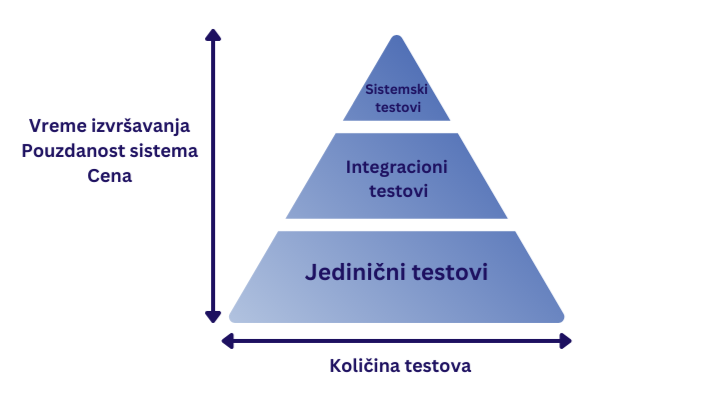
\includegraphics[width=0.8\textwidth]{piramidanova.png}
  \caption{Model piramide testiranja}
\end{figure}

\subsubsection{Testovi jedinica koda}
\par Jedinica je mala logička celina koda: može biti funkcija, klasa, metod klase, modul i slično. Jedinični test proverava samo da li se data jedinica ponaša prema svojoj specifikaciji. Ovi testovi se mogu pisati u potpunoj izolaciji, i ne zavise ni od jedne druge komponente, servisa, ni korisničkog interfejsa. Dakle, izdvajaju se najmanji testabilni delovi aplikacije i proverava se da li rade ono za šta su namenjeni. Ovi testovi su najjednostavniji za pisanje jer se bave malim delom aplikacije, te je k$\hat{o}$d koji se testira najčešće vrlo jednostavan. 
\par Pri dizajniranju jediničnih testova, nephodno je razmišljati o sledećim ciljevima: 
\begin{enumerate}
\item Dokazati da k$\hat{o}$d radi ono za šta je namenjen
\item Sprečiti greške --- izmena jednog dela koda može izazvati grešku u nekom drugom delu
\item Utvrditi lokaciju dela koda koji izaziva grešku
\item Napisati najmanju moguću količinu koda za testiranje
\end{enumerate}

\subsubsection{Anatomija jediničnih testova}
\par Kako bi k$\hat{o}$d jediničnog testa bio čitljiv i jednostavan za razumevanje, obrazac četvorofaznog testa (eng. \emph{four-phase test}) predlaže strukturu testa koja podrazumeva ne više od četiri faze \cite{4phase}. Svaki test jedinice koda se može podeliti na četiri jasno odvojive celine:  
\begin{enumerate}
\item Priprema (eng. \emph{setup}) --- sređivanje podataka koji će se prosleđivati pred samu proveru, često nije neophodna u testiranju čisto funkcionalnih programa.
\item Delovanje (eng. \emph{exercise}) --- pozivanje koda koji se testira, ključni deo svakog testa.
\item Verifikacija (eng. \emph{verify}) --- često deo prethodne faze, u ovom delu testovi proveravaju ponašanje koda. 
\item Rušenje (eng. \emph{teardown}) --- vraćanje podataka na prvobitno stanje, npr. ako se u prvoj fazi koriste neka deljena stanja, kao što je baza podataka. Ovaj korak se često izvršava implicitno. 
\end{enumerate}

\par Konkretan primer ovako organizovanog testa u programskom jeziku Elm dat je u primeru \ref{lst:4ph}. Definisan je jednostavan test, koji proverava da li funkcija koja sabira dva broja daje ispravan rezultat. U fazi pripreme brojevima i njihovoj očekivanoj sumi se dodeljuju vrednosti . U fazi delovanja poziva se funkcija \emph{sum}, a pozivanjem funkcije \emph{expect} proverava se da li je rezultat jednak očekivanom u fazi verifikacije. Faza rušenja u ovom slučaju ne treba da uradi ništa, te jednostavno vraća ().

\begin{lstlisting}[language=elm, caption={Četiri faze jediničnog testa},captionpos=b, label={lst:4ph}]
import Test exposing (..)

sumTest : Test
sumTest =
    describe "sum" [
      test "should add two numbers correctly" <| \() -> 
        let
        --Setup
           x = 2
           y = 3
           expected = 5
        in
        -- Exercise (sum)
        -- Verify (expect)
           expect (sum x y) |> toEqual expected
    ]

   -- Teardown
   teardown : Int -> ()
   teardown _ =
    ()
\end{lstlisting}

\subsubsection{Integracioni testovi}
\label{sec:integration}
\par Jedan od ključnih koraka u razvoju softvera jeste pisanje integracionih testova. Oni utvrđuju da li različite komponente sistema rade zajedno na predviđen način. Pojedinačni moduli i komponente se kombinuju i testiraju kao jedna celina. Cilj integracionog testiranje jeste identifikacija i rešavanje problema koji mogu nastati nakon što se komponente softverskog sistema integrišu i krenu da međusobno komuniciraju. Svaka od njih pojedinačno možda radi kako treba, ali nakon što se to utvrdi jediničnim testovima, potrebno je proveriti da li će njihova interakcija izazvati neželjeno ponašanje. 
\par U zavisnosti od potreba konkretnog sistema, postoje različiti pristupi integracionom testiranju. Ako su komponente viših nivoa kritične za funkcionalnost sistema, ili od njih zavisi mnogo drugih komponenti, ima smisla prvo testirati njih, pa kasnije postepeno preći na komponente nižih nivoa. Ovakav pristup se naziva testiranje odozgo nadole (eng. \emph{top-down integration testing}). U suprotnom, ako su komponente nižih slojeva arhitekture kritičnije za celokupan sistem, predlaže se testiranje odozdo nagore (eng. \emph{bottom-up integration testing}). Hibridno integraciono testiranje (eng. \emph{hybrid integration testing}) podrazumeva kombinaciju prethodna dva --- započinje sa testovima komponenti najvišeg sloja, zatim se prelazi na testiranje najnižeg sloja, sve dok se postepeno ne stigne do središnjih. Kada je sistem relativno jednostavan i ne postoji veliki broj komponenti, može se primeniti pristup po principu ''velikog praska'' (eng. \emph{big-bang integration testing}), koji podrazumeva testiranje svih komponenti odjednom, kao jedne celine. 
\par Ako se komponente nalaze u okviru istog sistema, gde postoji kontrola i neko očekivano ponašanje --- integracioni testovi su prilično jednostavni. Međutim, kada su u pitanju spoljašnje komponente i testiranje interakcije sistema sa njima, pisanje integracionih testova postaje malo komplikovanije. Mnoge aplikacije koriste baze podataka, druge servise ili API-je, sa kojima se testovi moraju uskladiti. U testovima se mogu koristiti pravi podaci, ili se umesto njih ubaciti takozvani dubleri (eng. \textit{test doubles}).
\par Integraciono testiranje je neophodno da bi se obezbedio kvalitetan i pouzdan softver, i zahvaljujući njemu rano se uočavaju različiti problemi do kojih može doći i time značajno redukuje vreme i cena celokupnog razvoja. 


\subsubsection{Sistemski testovi}
\label{sec:system}
\par Nakon završenog jediničnog i integracionog testiranja, neophodno je sprovesti sistemske testove. Ova vrsta testiranja se vrši nad kompletno integrisanim sistemom, i podrazumeva proveru da li celokupni sistem ispunjava zahteve, odnosno da li je spreman za isporuku krajnjim korisnicima. Sistemski testovi se sprovode u okruženju koje je konfigurisano tako da bude što sličnije onom kakvo će biti u produkciji. Praksa je da ih pišu testeri koji nisu učestvovali u razvoju, kako bi se izbegla pristrasnost. Pored funkcionalnih i nefunkcionalnih specifikacija koje se tiču ponašanja sistema, testiraju i očekivanja korisnika. Mogu biti manuelni ili automatski. 
\par Sistemsko testiranje se smatra testiranjem crne kutije (eng. \emph{black-box testing}). Ponašanje sistema se evaluira iz ugla korisnika, što znači da ne zahteva nikakvo znanje o unutrašnjem dizajnu i strukturi koda. Ono što je neophodno jeste da očekivanja i zahtevi budu precizni i jasni, kao i da se razume upotreba aplikacije u realnom vremenu. 
\par Postoji mnogo vrsta sistemskog testiranja, i potrebno je doneti odluku koje od njih će biti sprovedene, u zavisnosti od zahteva, tipa aplikacije i raspoloživih resursa. Neke od vrsta sistemskog testiranja su: 
\begin{itemize}
\item Testiranje oporavka (eng. \emph{recovery testing}) --- nakon što se izazove pad sistema, proverava se da li se on vraća u prvobitno stanje na ispravan način.
\item Testiranje perfomansi (eng. \emph{perfomance testing}) --- proverava se skalabilnost, pouzdanost, i vreme odgovora sistema.
\item Testiranje sigurnosti (eng. \emph{security testing}) --- proverava se da li je sistem adekvatno zaštićen od upada ili gubitka podataka. 
\item Regresiono testiranje (eng. \emph{regression testing}) --- proverava se da li su se pojavile neke naknadne greške pri dodavanju novih funkcionalnosti. 
\item Testiranje kompatibilnosti (eng. \emph{compatibility testing}) --- proverava se da li sistem radi ispravno u različitim okruženjima, npr. kada se koristi na drugom hardveru ili operativnom sistemu.
\end{itemize}
\par Pisanjem sistemskih testova obezbeđuje se kvalitet i pouzdanost softvera, umanjuje rizik od neispravnosti i povećava zadovoljostvo korisnika sistema. Temeljnim testiranjem sistema mogu se otkriti i ispraviti novi problemi pre samog puštanja u rad, koje nije bilo moguće primetiti u ranijim fazama testiranja. 

\section{Testiranje funkcionalnih programa}

\par Najvažnija stvar kod testiranja u funkcionalnoj paradigmi jeste pisanje čistih funkcija i njihovo testiranje u izolaciji, kako bi se obezbedila ispravnost i robustnost. Takođe je važno da se ne testira samo uspešan scenario, već i granični slučajevi, kao i slučajevi greške.

\subsection{Testiranje čistih funkcija}

\par Najjednostavniji k$\hat{o}$d za testiranje jeste čista funkcija. Pri testiranju čiste funkcije, s obzirom da ne postoje propratni efekti, test može da se fokusira samo na dve stvari: ulazne podatke i na sam izlaz funkcije. 
\par Kada je u pitanju čista funkcija, jedina priprema koja je potrebna jesu podaci koji će se proslediti kao parametri. Drugi korak jeste poziv funkcije, sa prosleđenim argumentima. Faza verfikacije su samo provere nad rezultatom, i samo nad rezultatom. Testovi su veoma jednostavni jer ne moraju da brinu o propratnim efektima i njihovim neželjenim posledicama, i uvek će dobijati  isti odgovor od testiranog koda, ma koliko puta bili pokrenuti. 
\par Aplikacije se u većini slučajeva neće sastojati od isključivo čistih funkcija, i u vezi sa tim postoje dve strategije \cite{testingelixir}. Prva je izdvojiti logiku u čiste funkcije, a druga dizajnirati funkcije tako da koriste neku od metoda ubrizgavanja zavisnosti (eng. \textit{dependency injection}) \footnote{Ubrizgavanje zavisnosti je obrazac u kom objekat ili funkcija prihvata druge objekte ili funkcije od kojih zavisi. Jedan od oblika inverzije kontrole, za cilj ima da razdvoji konstrukciju i upotrebu objekata i time smanjuje spregnutost programa.}, što omogućava izolaciju koda.

\subsubsection{Refaktorisanje ka čistim funkcijama} 
Ako je neki deo koda komplikovan za testiranje, najlakši način da se pojednostavi jeste refaktorisati ga u čistu funkciju, ukoliko je to moguće. Deo koda koji zavisi od nekog drugog dela iz spoljašnjosti će u većini slučajeva pozivati tu spoljašnju zavisnost i onda manipulisati rezultatom pre nego što vrati svoj rezultat. Što više takve manipulacije ima, to je taj deo koda bolji kandidat za premeštanje logike unutar čiste funkcije. Na slici \ref{fig:dep} su date vizuelne reprezentacije kako ovaj proces izgleda pre i posle izmeštanja koda u čistu funkciju. 
Na početku, funkcija može biti komplikovana za testiranje. Svaki test, za svaki mogući način ponašanja bi nekako morao da garantuje da druga funkcija (ona od koje zavisi prva) vraća neki očekivani odgovor. Ideja je da se deo logike (na slici označen sa ``manipulacija podataka ``) izvuče van --- u novu, čistu funkciju. Tako postaje zasebna komponenta, koja se može odvojeno lako testirati. Kada je taj deo logike dobro istestiran, može se smatrati sigurnim da se ponovo pozove u originalnoj funkciji. Zna se da će taj čisti k$\hat{o}$d uvek vraćati isti rezultat, i može se značajno redukovati broj testova neophodnih za testiranje originalne funkcije. U primeru koda... TODO primer

\begin{figure}[!ht]
  \centering
  \label{fig:dep}
  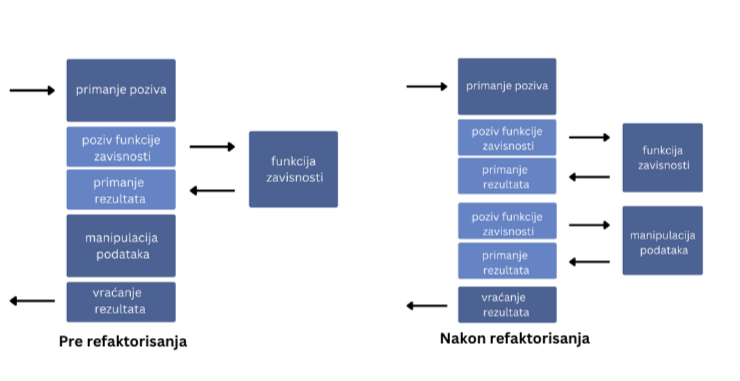
\includegraphics[width=0.9\textwidth]{dep.png}
  \caption{Izmeštanje koda u čistu funkciju}
\end{figure}

\par  U nekim slučajevima, nije lako odrediti šta se može izdvojiti u zasebnu funkciju. Tada postoji druga opcija za kreiranje kontrolisanog okruženja: napraviti zamenu za funkciju zavisnosti, i time izolovati k$\hat{o}$d. 

\subsection{Izolovanje koda} 
\par Ubrizgavanjem zavisnosti i kreiranjem dublera moguće je eliminisati spoljašnje promenljive, i time kontrolisati situaciju u kojoj k${o}$d koji se testira mora da se nađe. Tako se omogućava očekivanje nekog konkretnog rezultata. 
\par Zavisnost je bilo koji k$\hat{o}$d na koji se originalni k$\hat{o}$d oslanja. Korišćenjem DI (skraćenica za Dependency Injection) u testovima se kreiraju zamene zavisnosti koje se ponašaju na predvidljiv način, pa testovi mogu da se fokusiraju na logiku unutar koda koji se testira. U jediničnim testovima, najčešće se ubrizgava zavisnost tako što se prosledi kao parametar. Taj parametar može biti funkcija ili modul. Ubrizgavanje zavisnosti kroz API\footnote{skraćenica za aplikacioni veb interfejs (eng. \textit{web applicatoin
programming interface} )} obezbeđuje čist k$\hat{o}$d i jednostavne i kontrolisane jedinične testove. Sa druge strane, integracioni testovi zahtevaju drugačije metode ubrizgavanja zavisnosti. TODO nastavak...

% ------------------------------------------------------------------------------

\chapter{Portal MSNR}
\label{chp:msnr}

\par K$\hat{o}$d aplikacije pod nazivom \emph{Portal MSNR} koja će biti testirana javno je dostupan na \emph{GitHub-u} \cite{msnr-portal}. Portal MSNR je veb aplikacija namenjena praćenju i upravljanju aktivnostima kursa \emph{Metodologija stručnog i naučnog rada} \cite{rad}. Studenti na ovom kursu treba da steknu različite veštine koje se tiču pravilnog pisanja i recenziranja naučnih radova, pisanja CV-a, držanja prezentacija, i komunikacije u radu na timskim projektima. 

\section{Funkcionalnosti i osnovni entiteti portala}
\label{sec:entiteti}
\par Različite aktivnosti na kursu \emph{Metodologija stručnog i naučnog rada} implementirane su kao funkcionalnosti aplikacije. Korisnik portala može imati jednu od dve uloge: \emph{student} ili \emph{profesor}. Student na početku mora da podnese zahtev za registraciju, koju nakon toga odobrava profesor, i zatim student ima mogućnost da se prijavi na portal. Jedna od obaveza studenata na kursu jeste pisanje seminarskog rada --- profesor vrši odabir tema za tekuću godinu, a studenti treba da prijave svoju grupu za izradu seminarskog rada. Student ima i opciju da se prijavi za recenziranje radova drugih studenata, ukoliko to želi. Drugi zadatak koji se očekuje od studenata jeste pisanje CV-a. U okviru portala, student može priložiti tri različite vrste dokumenata --- prvu verziju seminarskog rada, recenzije, i svoju prvu verziju CV-a. Profesor, pored toga što vrši pregled zahteva za registraciju i odabir tema, ima mogućnost dodavanja svih aktivnosti tokom godine, i na kraju --- njihovo ocenjivanje.

\subsection{Entiteti}
\par Osnovni entiteti aplikacije predstavljeni su tabelama u bazi podataka i relacijama između njih.  Polazni entiteti su \emph{zahtev za registraciju studenata}, \emph{korisnik} i \emph{semestar}. U tabeli korisnika inicijalno postoji jedan nalog koji ima rolu profesora, a pri odobravanju registracije studenta kreira se nalog sa rolom studenta, i studentu se šalje elektronska pošta sa vezom za postavljanje lozinke. Pored unosa u tabelu \textit{users}, vrše se unosi u još dve tabele: \emph{students}, koja sadrži referencu ka korisniku i \emph{students{\textunderscore}semesters}, koja predstavlja relaciju između studenta i semestra, a ima i referencu ka tabeli \emph{groups} --- svaki student u toku jednog semestra može pripadati jednoj grupi. Nakon što profesor odabere teme za seminarske radove, vrši se unos u tabelu \emph{topics}, koja ima referencu ka semestru u kom se mogu odabrati. Prethodno navedeni tipovi aktivnosti predstavljeni su tabelom \emph{activity{\textunderscore}types}, a tabela \emph{activities} predstavlja relaciju između tipa aktivnosti i semestra. Tabela \emph{assignments} odnosi se na dodeljene aktivnosti koje mogu biti grupne ili individualne, te može imati referencu ka studentu ili ka grupi. Većina dodeljenih aktivnosti podrazumeva predaju dokumenata, koji će se nalaziti na serveru, a informacije o predatim dokumentima čuvaju se u tabeli \emph{documents}. Ova tabela sadrži referencu ka korisniku koji je priložio dokument, a tabela \emph{assignments{\textunderscore}documents} vezuje dokument i dodeljenu aktivnost.
\par Spisak naziva entiteta i tabela u okviru baze podataka koje njima odgovaraju dati su u tabeli \ref{tab:1}. Svaki od ovih entiteta, kao i relacije između njih, biće pojedinačno istestirani u narednom poglavlju.

\begin{table}[htb]
\centering
\caption{Entiteti portala i odgovarajuće tabele u bazi}
\label{tab:1}
\begin{tabular}{ |c|c| } 
 \hline
\textbf{Entitet} & \textbf{Tabele u bazi podataka} \\ 
 \hline
\textit{\textbf{Zahtev za registraciju studenata}} & \emph{student{\textunderscore}registrations}  \\ 
\textit{\textbf{Korisnik}} & \emph{users}  \\ 
\textit{\textbf{Semestar}} & \emph{semesters}  \\ 
\textit{\textbf{Student}} & \emph{students} i  \emph{student{\textunderscore}semester} \\ 
\textit{\textbf{Grupa}} & \emph{groups}  \\ 
\textit{\textbf{Tema seminarskog rada}} & \emph{topics}  \\
\textit{\textbf{Aktivnost}} & \emph{activities}  \\
\textit{\textbf{Tip aktivnosti}} & \emph{activity{\textunderscore}types} \\   
\textit{\textbf{Dodeljene aktivnosti}} & \emph{assignments}  \\
\textit{\textbf{Dokument}} & \emph{documents} i  \emph{assignments{\textunderscore}documents} \\
 \hline
\end{tabular}
\end{table}

\section{Arhitektura portala}
\par Portal MSNR je primer klijent/server aplikacije koja se sastoji od tri sloja. Klijentski sloj implementiran je u programskom jeziku \emph{Elm}, kao jednostranična aplikacija (eng. \emph{Single Page Application --- SPA}) koja predstavlja korisnički interfejs. U sredini se nalazi aplikacioni veb interfejs koji je implementiran u \emph{Elixir} programskom jeziku pomoću razvojnog okvira \emph{Phoenix}, u stilu arhitekture \emph{REST} (eng. \emph{Representational State Transfer}) \cite{rest}. Treći sloj predstavlja relaciona baza podataka, i sistem za upravljanje bazom \emph{PostgreSQL} \cite{postgre}. Slika \ref{fig:msnr-arch} prikazuje navedenu arhitekturu. 

\begin{figure}[!ht]
  \centering
  \label{fig:msnr-arch}
  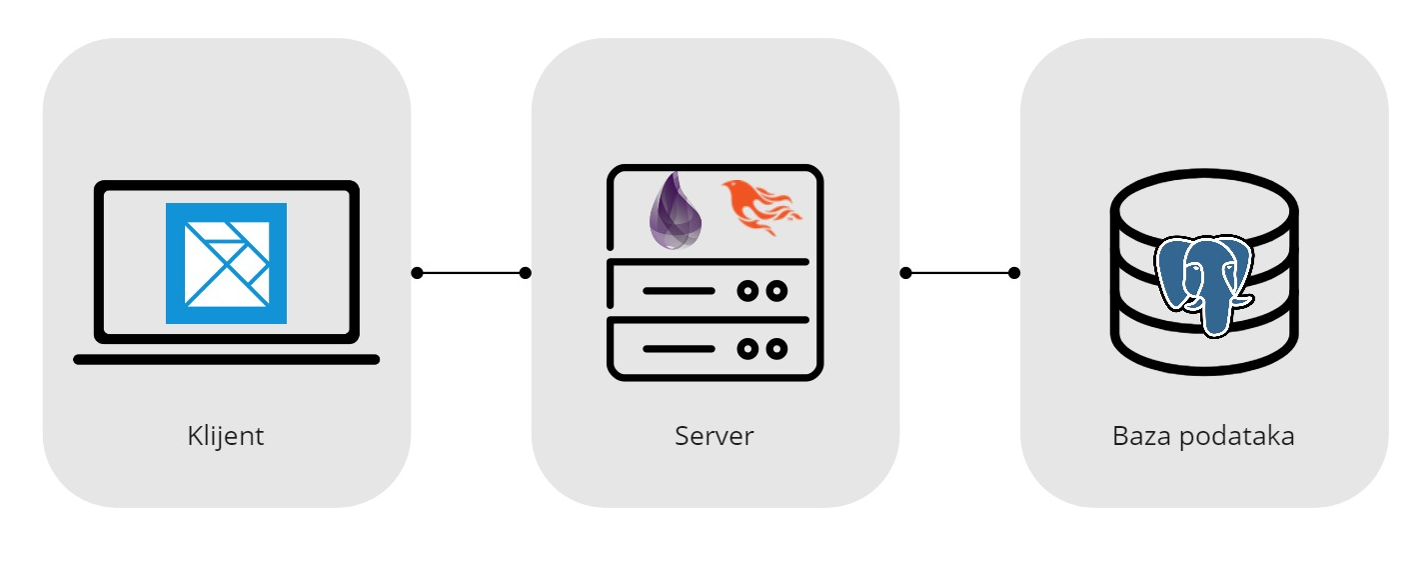
\includegraphics[width=0.9\textwidth]{msnr-arch.png}
  \caption{Arhitektura Portala MSNR \cite{rad}}
\end{figure}

\par Testiranje ovakve aplikacije podrazumeva podelu na različite vrste testova. Za početak, jedinični testovi koji se odnose na individualne funkcije i upravljače koji barataju zahtevima u okviru serverskog dela aplikacije moraju biti napisani u programskom jeziku Elixir. Na serverskoj strani, potrebno je napisati i testove koji simuliraju zahteve API-ju i verifikuju odgovore od baze. Sa druge strane, jedinični testovi koji se fokusiraju na pojedinačne komponente i funkcije korisničkog interfejsa moraju biti napisani u Elm programskom jeziku. Nakon pojedinačnog testiranja klijentske i serverske aplikacije, slede integracioni testovi koji proveravaju kako korisnički interfejs funkcioniše zajedno sa API-jem. Na kraju je neophodno testirati celokupan sistem, od korisničkog interfejsa do baze podataka, pisanjem sistemskih testova. S obzirom na to da se radi o veb aplikaciji, mogu se sprovesti i testovi opterećenja koji će proveriti kako portal podnosi velike količine zahteva i korisnika.

\chapter{Testiranje serverskog dela aplikacije}
\label{chp:elixir}

\par Razvojni okvir \emph{Phoenix} koristi se za razvoj veb aplikacija u programskom jeziku Elixir \cite{phx}. Zasnovan je na obrascu \emph{model-pogled-upravljač} (eng. \emph{Model-View-Controller pattern, MVC}). Serverski deo aplikacija MSNR portal implementiran je kao \emph{Phoenix} projekat. Preciznije, projekat je u osnovi \emph{Mix} projekat, sa \emph{Phoenix} proširenjima. Pored konfiguracione datoteke \emph{mix.exs}, i direktorijuma \emph{lib} koji sadrži osnovni k$\hat{o}$d aplikacije, kreira se i direktorijum \emph{test}. Unutar ovog direktorijuma će biti smešteni svi testovi vezani za serversku stranu aplikacije. 
\par K$\hat{o}$d napisan u Elixir-u zavisi od nekoliko Erlang biblioteka. Međutim, kada je testiranje koda u pitanju, alati i biblioteke koji se koriste su jedinstveni za svaki od ova dva jezika. Ovde će se govoriti o testiranju isključivo Elixir koda. 
\par Zajedno sa ovim jezikom dolazi njegov razvojni okvir za testiranje, \emph{ExUnit} \cite{exunit}. U ovom poglavlju biće predstavljeni različiti koncepti testiranja u programskom jeziku Elixir, kroz pisanje testova za serverski deo aplikacije MSNR portal. 

\section{Testiranje jedinica koda u programskom jeziku Elixir}
\label{sec:elixunit}

\textit{ExUnit} je Elixir-ov ugrađeni razvojni okvir koji ima sve što je neophodno za iscrpno testiranje koda i biće osnova za sve testove kroz ovo poglavlje. S obzirom na to da je Elixir funkcionalni jezik, može se diskutovati o tome šta se smatra "jedinicom". Uobičajeno je da se jedinični testovi fokusiraju na pojedinačnu funkciju i njenu logiku, kako bi se opseg testa održavao što užim, radi bržeg pronalaženja grešaka. Međutim, nekada ima smisla da se u opseg testa uključi više modula ili procesa, i time se proširi definicija jedinice koda. Znati kada treba proširiti taj opseg može pozitivno uticati na jednostavnost i održavanje samih testova. 
\par Pisanje testova u programskom jeziku Elixir je moguće bez potrebe za drugim bibliotekama, jer je \emph{ExUnit} razvijan zajedno sa samim jezikom od početka. Svi testovi su implementirani kao Elixir skripte, pa je pri davanju imena testu neophodno koristiti ekstenziju datoteke \emph{.exs}. Pre pokretanja testova potrebno je pokrenuti \emph{ExUnit}, kao što je prikazano u primeru koda \ref{lst:start}. Ova naredba se obično navodi unutar automatski generisane datoteke \emph{test/test{\textunderscore}helper.exs}. 

\begin{lstlisting}[language=elixir, caption={Pokretanje ExUnit},captionpos=b, label={lst:start}]
# test/test_helper.exs

ExUnit.start()
\end{lstlisting}

\par Testovi se pokreću najpre pozicioniranjem u direktorijum projekta, a zatim navođenjem komande \emph{mix test}. Ova komanda pokreće sve testove koji se nalaze unutar \emph{test} direktorijuma. Navođenjem parametra \emph{--only} i imena testa ili modula može se pokrenuti specifičan test ili skup testova unutar jednog modula. Pozivanje naredbe \emph{mix test} pokreće testove, i daje sledeći izlaz:  

\begin{lstlisting}[style=DOS]
PS C:\Users\panap\testing-msnr-portal\portal\msnr_api> mix test

..............
Finished in 0.2 seconds (0.00s async, 0.2s sync)
16 tests, 0 failures
\end{lstlisting}


\par Svita testova (eng. \emph{test suite}) je kolekcija testova slučajeva upotrebe, koji imaju isti posao, ali različite scenarije. Ona može služiti kao dokumentacija, sa opisima o očekivanom ponašanju koda, tako da treba voditi računa da bude dobro organizovana. \emph{ExUnit} dolazi sa veoma korisnim funkcijima i makroima koji omogućavaju tu organizaciju u jednu čitljivu i održivu  datoteku. Alat \emph{describe} omogućava davanje opisa grupe testova, kao i dodeljivanja zajedničke pripreme podataka za celu grupu. Preporuka je za početak grupisati testove po funkciji, kao što je prikazano u primeru koda \ref{lst:desc}, ali odluka o načinu grupisanja je na pojedincu. Svrha je čitljivost i lakše razumevanje. 

\begin{lstlisting}[language=elixir, caption={Opisivanje testova unutar jedne grupe},captionpos=b, label={lst:desc}]
defmodule MyApp.ModuleTest do 
   use ExUnit.Case 
   
   describe ''thing_to_do/1'' do
   	test ''it returns :ok, calls the function if the key is correct''
   	test ''it does not call the function if the key is wrong''
   end
end
\end{lstlisting}

\par Testovi u Elixir projektima se organizuju u module i test slučajeve. U prethodnom primeru koda, modul pod nazivom \emph{ModuleTest} se sastoji od dva test slučaja. Navođenjem ključne reči \emph{test}, a za njom niske koja treba da opiše šta je to što test treba da uradi, definiše se jedna funkcija koja predstavlja test slučaj.
\par Za svaku funkciju ili upravljač potrebno je napisati test slučajeve. Unutar jednog test slučaja poziva se funkcija ili upravljač i proverava se očekivani rezultat. Makroom \emph{assert} se testira da li je izraz istinit. U slučaju da nije, test ne prolazi i izbacuje grešku. Korišćenje ovog makroa može se videti u primeru \ref{lst:hello}.  Ako funkcija \emph{hello} definisana unutar modula \emph{Example} kao povratnu vrednost vraća atom \emph{:world}, ovaj test prolazi.

\begin{lstlisting}[language=elixir, caption={Testiranje jednostavne funkcije},captionpos=b, label={lst:hello}]
defmodule HelloTest do
    use ExUnit.Case
    doctest Example
    
    test ''function returns expected atom'' do
    	assert Example.hello() == :world
    end
end
\end{lstlisting}

\par U slučaju da leva i desna strana izraza navedenog nakon makroa \emph{assert} nisu jednake, test ne prolazi, a \emph{ExUnit} daje obaveštenje o tome koji od testova su neuspešni, kao i koje su prava i očekivana vrednost. Ako se umesto \emph{:world} u testu navede na primer atom \emph{:word}, test ne prolazi i dobija se sledeći izlaz:

\begin{lstlisting}[style=DOS]
1) function returns expected atom (HelloTest)
     test/hello_test.exs:5
     Assertion with == failed
     code:  assert Example.hello() == :word
     left:  :world
     right: :word
     stacktrace:
       test/helllo_test.exs:6 (test)

.

Finished in 0.04 seconds
2 tests, 1 failures
\end{lstlisting}

\par U narednoj listi, navedeni su neki od makroa koji se koriste u testovima, pored makroa \emph{assert}: 
 \begin{itemize}
 \item \emph{refute} --- koristi se kada je potrebno utvrditi da je izraz uvek neistinit. 
 \item \emph {assert{\textunderscore}raise} --- koristi se kada je potrebno proveriti da li se javlja konkretan izuzetak.
 \item \emph{assert{\textunderscore}receive} --- koristi kada je potrebno proveriti da li je proces primio konkretnu poruku.
 \item \emph {capture{\textunderscore}io} --- koristi se kada je potrebno proveriti da li se na standardanom izlazu ispisuje očekivano.
 \item \emph{capture{\textunderscore}log} --- koristi se kada je potrebno proveriti sadržaj log poruka, npr. pri pozivu \emph{Logger.info}.
 \item \emph{setup i setup{\textunderscore}all} --- koriste se kada je potrebno izvršiti pripremu testova, pokreću se pre svakog testa, ili pre jedne grupe.
 \end{itemize}
 
 \par

\section{Testiranje komunikacije sa bazom podataka}
\par \emph{Ecto} biblioteka zadužena je za sve interakcije sa relacionim bazama podataka u Elixir okruženju \cite{ecto}. Pored komunikacije sa bazom, \emph{Ecto} ima i ulogu u validaciji. U ovom delu, prikazani su testovi koji proveravaju da li k$\hat{o}$d koristi funkcionalnosti ove biblioteke na ispravan način. Dva značajna modula koja \emph{Ecto} poseduje su \emph{Ecto.Schema} i \emph{Ecto.Changeset}. Prvi se odnosi na definisanje mapiranja eksternih podataka u Elixir strukture. Koncept skupa promena (eng. \emph{changeset}) odnosi se na proces validacije podataka, njihovog konvertovanja i provere dodatnih uslova pre nego što se upišu u bazu. \emph{Ecto.Changeset} modul opisuje kako se menjaju podaci. 
\par Svi testovi koji se odnose na \emph{Ecto} biblioteku nalaze se u direktorijumu \textit{'/test/msnr{\textunderscore}api/schema'}, u okviru projekta \emph{msnr{\textunderscore}api}. 
\par Na početku, napisani su jednostavni testovi koji proveravaju ispravnost definisanja struktura pomoću \emph{Ecto.Schema} modula. Primer definisanja entiteta dodeljenih aktivnosti  dat je u primeru koda \ref{lst:schema}. Pomoću makroa \emph{schema} i \emph{field} definišu se tabele, njihova polja i relacije sa drugim tabelama. Oni istovremeno definišu i Elixir strukturu --- u slučaju primera \ref{lst:schema}, ta struktura se naziva \emph{Assignment}. 

\begin{lstlisting}[language=elixir, caption={Shema tabele assignments},captionpos=b, label={lst:schema}]
defmodule MsnrApi.Assignments.Assignment do
  use Ecto.Schema
  import Ecto.Changeset

  schema "assignments" do
    field :comment, :string
    field :completed, :boolean, default: false
    field :grade, :integer
    field :student_id, :id
    field :group_id, :id
    field :activity_id, :id
    field :related_topic_id, :id
    timestamps()
  end

  def changeset(assignment, attrs) do
    assignment
    |> cast(attrs, [:comment, :grade])
    |> validate_required([:comment, :grade])
  end
...
\end{lstlisting}

\subsection{Testiranje polja i tipova}
\par Test koji se odnosi na prethodni primer prikazan je u kodu \ref{lst:testschema}. Ovo je primer jednostavnog jediničnog testa koji proverava da li definisana shema ima tačna polja i odgovarajuće tipove. Unutar testa se prvo prolaskom kroz sva polja Assignment strukture izvuku polje i njegov tip, i zatim se navodi ključna reč \emph{assert}, kojom se proverava da li su prava polja i tipovi jednaki očekivanim. Lista \emph{@expected{\textunderscore}fields{\textunderscore}with{\textunderscore}types} definisana je kao lista parova polja i odgovarajućih tipova, kao što su navedeni u primeru \ref{lst:schema}. Unutar assert naredbe, i prava i očekivana lista pretvorene su u \emph{MapSet} strukturu, kako bi se redosledi polja poklapali sa obe strane. Slični testovi napisani su i za sve ostale entitete navedene u sekciji \ref{sec:entiteti}.

\begin{lstlisting}[language=elixir, caption={Test za proveru polja i tipova tabele assignments},captionpos=b, label={lst:testschema}]
defmodule MsnrApi.Schema.AssignmentTest do
  use ExUnit.Case
  alias MsnrApi.Assignments.Assignment
  
  describe "fields and types" do
    test "it has the correct fields and types" do
      actual_fields_with_types =
        for field <- Assignment.__schema__(:fields) do
          type = Assignment.__schema__(:type, field)
          {field, type}
    end
    
        assert MapSet.new(actual_fields_with_types) == MapSet.new(@expected_fields_with_types)
    end
  end
\end{lstlisting}


\subsection{Testiranje skupa promena}
\par Funkcija \emph{changeset} obuhvata manipulacije i transformacije podataka, kao i njihovu validaciju pre unosa u bazu podataka. Svrha ove funkcije je da svi podaci koji se unose ili ažuriraju u bazi budu ispravni i u skladu sa zahtevima aplikacije. Funkcija \emph{changeset/2} iz primera koda \ref{lst:schema} 


\section{Integraciono testiranje}
\label{sec:elixint}
\par Nakon dobro istestiranih pojedinačnih funkcija i modula, potrebno je proveriti da li komponente funkcionišu ispravno kao celina. U ovom poglavlju biće prikazani testovi koji proveravaju da li različiti delovi sistema koji komuniciraju međusobno, kao i sa nekim eksternim sistemima, rade to na ispravan način.

\subsection{Test dubleri}

\par 

\subsection{Neki podnaslov}
U aplikaciji MSNR portal --- TODO konkretni primeri ... 

\chapter{Testiranje klijentskog dela aplikacije}
\label{chp:elm}

\chapter{Testiranje celokupnog sistema --- End to End}
\label{chp:e2e}

\section{Integracija klijentske i serverske strane}

\section{Testiranje opterećenja}

% ------------------------------------------------------------------------------
\chapter{Zaključak}
% ------------------------------------------------------------------------------

% ------------------------------------------------------------------------------
% Literatura
% ------------------------------------------------------------------------------
\literatura

% ==============================================================================
% Završni deo teze i prilozi
\backmatter
% ==============================================================================

% ------------------------------------------------------------------------------
% Biografija kandidata
%\begin{biografija}

%\end{biografija}
% ------------------------------------------------------------------------------

\end{document}
